\documentclass[border=3pt,varwidth]{standalone}
\usepackage{amsmath,amssymb}
\usepackage{tikz}
\usetikzlibrary{arrows.meta,calc,decorations.markings,patterns,positioning,angles,quotes}
\tikzset{
  >=Stealth,
  every node/.style={font=\normalsize},
  wire/.style={line width=0.9pt},
  thinwire/.style={line width=0.6pt},
  fieldline/.style={line width=0.6pt,-{Stealth[length=2.2mm]}},
  axis/.style={line width=0.7pt,-{Stealth[length=2.2mm]}},
  dashedwire/.style={line width=0.9pt,dash pattern=on 3pt off 2pt},
  resistor/.style={line width=0.9pt},
  chargepos/.style={circle,draw,line width=0.8pt,minimum size=5mm,inner sep=0pt},
  dotcharge/.style={circle,fill,inner sep=0pt,minimum size=2.4pt}
}
% Draw a resistor box centered at (x,y) with width w, height h, horizontal
\newcommand{\resbox}[4]{%
  % #1=x #2=y #3=halfwidth #4=label
  \draw[resistor] (#1-#3,#2-0.18) rectangle (#1+#3,#2+0.18);
  \ifx\\#4\\\else\node[above=2pt] at (#1,#2+0.18) {#4};\fi
}
% Battery symbol: long thin line (+) then short thick line (-), centered at (x,y)
\newcommand{\battery}[2]{%
  % #1=x #2=y ; long line left=+, short line right=- by default orientation
  \draw[wire] (#1-0.09,#2-0.32) -- (#1-0.09,#2+0.32);
  \draw[line width=2.6pt] (#1+0.09,#2-0.16) -- (#1+0.09,#2+0.16);
}

\begin{document}
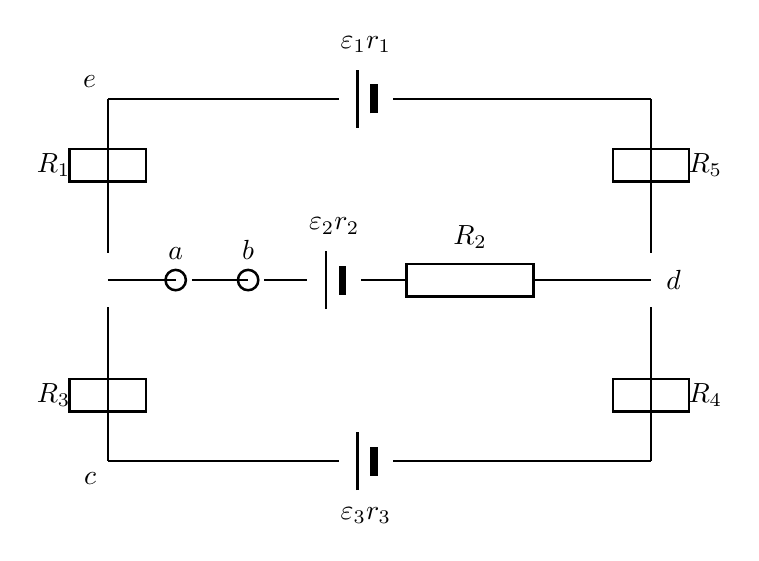
\begin{tikzpicture}[scale=1.15]
  % left column: e (top) - R1 - a/b node row (y=0) - R3 - c (bottom)
  \draw[wire] (0,2) -- (0,0.55);
  \resbox{0}{1.27}{0.42}{}
  \node[left=10pt] at (0,1.27) {$R_1$};
  \draw[wire] (0,0.55) -- (0,0.3);
  \draw[wire] (0,-0.3) -- (0,-0.55);
  \resbox{0}{-1.27}{0.42}{}
  \node[left=10pt] at (0,-1.27) {$R_3$};
  \draw[wire] (0,-0.55) -- (0,-2);
  \node[above left=1pt] at (0,2) {$e$};
  \node[below left=1pt] at (0,-2) {$c$};

  % right column: top-right - R5 - d - R4 - bottom-right
  \draw[wire] (6,2) -- (6,0.55);
  \resbox{6}{1.27}{0.42}{}
  \node[right=10pt] at (6,1.27) {$R_5$};
  \draw[wire] (6,0.55) -- (6,0.3);
  \draw[wire] (6,-0.3) -- (6,-0.55);
  \resbox{6}{-1.27}{0.42}{}
  \node[right=10pt] at (6,-1.27) {$R_4$};
  \draw[wire] (6,-0.55) -- (6,-2);
  \node[right=2pt] at (6,0) {$d$};

  % top branch: e -- battery eps1,r1 -- top-right corner
  \draw[wire] (0,2) -- (2.55,2);
  \battery{2.85}{2}
  \node[above] at (2.85,2.4) {$\varepsilon_1 r_1$};
  \draw[wire] (3.15,2) -- (6,2);

  % bottom branch: c -- battery eps3,r3 -- bottom-right corner
  \draw[wire] (0,-2) -- (2.55,-2);
  \battery{2.85}{-2}
  \node[below] at (2.85,-2.4) {$\varepsilon_3 r_3$};
  \draw[wire] (3.15,-2) -- (6,-2);

  % middle branch: open node a, open node b, battery eps2 r2, R2, to d
  \draw[wire] (0,0) -- (0.75,0);
  \draw[wire] (0.75,0) circle (3.2pt);
  \node[above] at (0.75,0.12) {$a$};
  \draw[wire] (0.93,0) -- (1.55,0);
  \draw[wire] (1.55,0) circle (3.2pt);
  \node[above] at (1.55,0.12) {$b$};
  \draw[wire] (1.73,0) -- (2.2,0);
  \battery{2.5}{0}
  \node[above] at (2.5,0.4) {$\varepsilon_2 r_2$};
  \draw[wire] (2.8,0) -- (3.3,0);
  \resbox{4.0}{0}{0.7}{$R_2$}
  \draw[wire] (4.7,0) -- (6,0);
\end{tikzpicture}
\end{document}
